\documentclass[12pt,english,twocolumn]{revtex4}

\usepackage{babel,bbm,graphicx,eurosym,amsmath,revsymb,amssymb,gensymb}
\usepackage[utf8]{inputenc}

\usepackage{enumerate}
\usepackage{lipsum}
\usepackage{float}
\usepackage{filecontents}
\usepackage{dsfont}
\usepackage{subcaption}
\usepackage{hyperref}
\usepackage{chemfig}
\captionsetup{compatibility=false}
\bibliographystyle{unsrtnat}
%\usepackage{biblatex}
%\addbibresource{./references.bib}

\usepackage{ wasysym }
\usepackage{afterpage}
\usepackage{makecell}


\jot4mm
\parskip2ex
\parindent0mm
\renewcommand{\baselinestretch}{1.1}
\hbadness=10000
\clubpenalty10000
\widowpenalty10000
\displaywidowpenalty=10000


\newcommand{\nocontentsline}[3]{}
\newcommand{\tocless}[2]{\bgroup\let\addcontentsline=\nocontentsline#1{#2}\egroup}




\begin{document}
\title{How to choose and adjust the tracing parameters}

\maketitle
\makeatletter\onecolumngrid@push\makeatother

\tableofcontents
\newpage

\makeatletter\onecolumngrid@pop\makeatother
\newpage
\clearpage
\section{Choosing tracing parameters} \label{sec:input_params}
The algorithm requires the specification of several parameters used during the tracing that also strongly impact the tracing result. These parameters have to be chosen sensibly in order to obtain a sufficiently accurate fiber tracing. Here, these parameters are referred to as $\sigma_{conv}$, $r_{min}$, $r_{max}$, $\sigma_{smooth}$, $steps$, $thresh$, $r_{step}$ and $min\_loop\_length$. Their exact function is described in \ref{sec:math_basis} to \ref{sec:closures}, but here a general overview of how to find sensible values for them is given. Since this algorithm could be applied to a wide variety of fibrous systems and imaging techniques, it is hard to speculate on what values would work best in each case. So far the algorithm has only been applied to SEM images and the guidelines given here are based on the experience gathered on those images. In general it was possible to find one set of parameters that works well on one kind of image. Therefore the results of similar images are very comparable since they can be analyzed with the same set of parameters. Also one or more parameters could be adjusted within a considerable range while maintaining a decent tracing quality. It has also proven sometimes useful, to completely disregard the following guidelines to obtain a sufficient tracing quality. The algorithm has also been designed to be scale invariant. This means, that if a image is magnified or the resolution is increased, the tracing should be almost identical if the parameters are adjusted accordingly. Some parameters have to be scaled linearly while others can stay constant if the scale of the image to be traced changes. The parameters whose range is recommended relative to the fiber diameter have to be scaled linearly with the magnification of the image. All other parameters do not need to be changed.\\


$\sigma_{conv}$ should be chosen at around half the fiber diameter. It determines the amount of smoothing before the computation of the hessian matrix. A function has been implemented to map each pixel tho the smaller eigenvalue of its Hessian, flip the sign and optionally color code the fiber direction (See figure \ref{fig:-lambda1_vs_og} or \ref{fig:-lambda1_vs_og_1}). The resulting image only depends on $\sigma_{conv}$ and serves to adjust it. If $\sigma_{conv}$ is chosen to small, the edges of the fiber will be brighter than its center. If $\sigma_{conv}$ is chosen to big, the fibers will seem washed out and blurry. If $\sigma_{conv}$ is chosen correctly, some structure should be visible in the fibers and the center of them should be brightest part of the image. There also should not be any visible noise left. In the tracing, a $\sigma_{conv}$ that is to small can be one cause for multiple tracings of one fiber. The tracing with a $\sigma_{conv}$ that is chosen to big, will have some fibers not traced, or bundles of them only traced once.\\


$r_{min}$ is typically chosen as 0, but sometimes a value around or less than half fiber diameter can improve the tracing. It determines the minimal distance between the node and the pixels it considers for the angle of the newly spawned node.\\


$r_{max}$ is one of the most challenging parameters to adjust, since it does not strongly impact the amount of branches and there is no additional metric by which to judge its choice. Although the sensible range varies, a usable starting point seems to be twice the fiber diameter or slightly more than that. If there are many branches not being traced, $r_{max}$ might be to small. On the other hand, if the tracing of a fiber seems to strongly influenced by the surrounding fibers, $r_{max}$ is likely to big. It determines the maximal distance between the node and the pixels it considers for the angle of the newly spawned node. Big values of $r_{max}$ increase the computation time, since more pixels have to be considered.\\


$\sigma_{smooth}$ directly impacts the amount of new nodes spawned. The lower $\sigma_{smooth}$, the more nodes will be spawned. 0.5 radians appears to be a sensible starting value independent of the fiber diameter. It should not be chosen much higher than 0.8 radians and not lower than 0.35 radians. $\sigma_{smooth}$ is responsible for the smoothing of the angle dependent curvature. The local maxima of this smoothed function determine the directions new nodes are spawned in. If the smoothing is stronger with a bigger $\sigma_{smooth}$, close local maxima will unite to one single local maxima, and only one new node will be spawned instead of several. If to many nodes are spawned, and they lie angularly close to each other, $\sigma_{smooth}$ will likely have to be increased. If not enough branches are being found, $\sigma_{smooth}$ might be to big.\\


$steps$ is not a very important variable. It is mostly a trade off between run time and angular resolution. It determines the amount of points for which the smoothed angle dependent function is evaluated. Therefore it determines the amount of possible angles in which new nodes can be spawned. If the value is not chosen so low, that not all local maxima are captured, only small decreases in tracing quality will be caused. Values often chosen for it here were 100 and 360.\\


$thresh$ has a somewhat similar impact as $\sigma_{smooth}$. It to strongly impacts the amount of new nodes being spawned. $thresh$ determines the threshold above which local maxima in the smoothed angle dependent curvature are used to spawn new nodes. If a lot of nodes are spawned into noisy regions of the image where no fibers are present, $thresh$ likely has to be increased. It should be noted, that with lower $\sigma_{smooth}$, the local maxima will become higher and more likely reach above $thresh$. If no nodes are spawned at all, $thresh$ is likely the cause and has to be reduced. $thresh$ should never be chosen below zero. Zero is also a good starting point, from which $thresh$ can carefully be increased. A upper limit for $thresh$ can not really be generally given, since it varies a lot between different kinds of images. In gerneral, once a decent set of parameters has been found, it is a good idea to increase $thresh$ while simultaneously decreasing $\sigma_{smooth}$ or vice versa. This will cause the amount of spawned nodes to remain relatively constant, but change their positions.\\

$r_{step}$ is, similar to $steps$, somewhat of a trade of between run time and resolution. It determines how far away form the spawning node, new nodes will be placed. A smaller $r_{step}$ means, that more nodes have to be spawned for the same length of fiber. If it is chosen to big, the nodes can skip by branches of fibers, meaning that these branches will not be traced. It is however possible to choose $r_{step}$ to small. Especially when the fiber thickness exceeds 5 pixels, a to small value of $r_{step}$ might cause single fibers to be traced several times or even whole meshworks to be falsely traced on top of one single fiber. A sensible staring point is between half and full fiber thickness.\\

$min\_loop\_length$ is the minimal length of loops expressed in the amount of nodes part of the loop. A good range is between 5 and 10, and 7 appears as a usable starting value. Great care has to be taken since it can easily be used to manipulate results by allowing or not allowing smaller loop sizes in the tracing. A good idea is to find the extremes of its sensible range and choose the middle. If the parameter is chosen to small, a lot of unwanted connections will be generated, resulting in regions extreamly densely populated with connections. If this parameter is chosen to large, a lot of almost closed loops will be visible in the tracing.


\section{How the fiber tracing works}
\subsection{Desired tracing result and datastructure}
The aim is to trace all fibers on a grayscale image by populating the image with nodes that are connected to one another. The nodes should lie on fibers and the connections between them should run along fibers so that if we plot all the connections between the fibers, each fiber in the image has exactly one plotted line running along it and every plotted line is on a fiber. One node can be connected to an arbitrary amount of other nodes, allowing for branching of the traced network. The positions of nodes are not bound to pixel positions but can lie anywhere between the pixels of the image but not outside the image. The connections between nodes should also never cross. In the case of crossing fibers, a node connected with both fibers should be placed at the junction instead. These nodes are placed based on an algorithm described below that also takes several input parameters influencing the fiber tracing. These input parameters have to be adjusted based on the kind of image to be traced (See \ref{sec:input_params}).
\subsection{Mathematical basis} \label{sec:math_basis}
The algorithm works on the basis of the Hessian of the Gaussian transform to compute the smoothed second order derivatives of the image brightness profile (For more information see \ref{sec:how_to_derive_images} to \ref{sec:Hessian_usefulness}). The convolution with the three second order derivatives of the Gaussian yields the Hessian matrix in every pixel. Before this convolution, the image brightness is rescaled so the brightest pixel has a value of 255 and the darkest one a value of 0. Using the Hessian matrix, the directional second order derivative in any pixel and any direction can be easily computed. Generally negative second order derivatives with a big absolute value indicate the presence of a fiber. Also this fiber likely travels perpendicular to the direction of this directional second order derivative. Here the first input parameter of the algorithm is the standard deviation $\sigma_{conv}$ of the Gaussian whose second order derivatives are used to compute the hessian.
\subsection{Positioning of starting nodes}
The algorithm works by already existing nodes spawning new nodes. To kick start this process, at least one starting node has to be created. The starting node(s) should be placed on top of fibers or the tracing will likely terminate immediately. The placing of the starting node(s) can be done manually, but an automated function for this task has also been implemented. Its goal is to make sure, the placed nodes lie on fibers and are not clustered together to closely. It tries to achieve this by first computing the smaller eigenvalue of the hessian in each pixel and then flipping its sign. On top of a fiber, this smaller eigenvalue is negative and has a large absolute value, so when its sign is flipped this results in a large positive value. The values obtained this way generate a second greyscale image (See figure \ref{subfig:-lambda1_1}).
\begin{figure}[h!]
    \centering
    \begin{subfigure}[b]{\linewidth}
        \includegraphics[width=\linewidth]{illustrations/og_image.png}
        \caption{SEM image of actin fibers. Imaged by Daniel Flormann.}
        \label{subfig:og1_1}
    \end{subfigure}
    \begin{subfigure}[b]{\linewidth}
        \includegraphics[width=\linewidth]{illustrations/og_viz_grey.png}
        \caption{$-1$ times the smaller eigenvalue of the Hessian matrix in each pixel of figure \ref{subfig:og1_1} is mapped to the brightness in the corresponding pixel.}
        \label{subfig:-lambda1_1}
    \end{subfigure}
    \caption{Using the eigenvalues of the Hessian to remove noise and enhance fiber visibility. The Hessian is computed using the second order derivatives of a Gaussian filter. Then the smaller eigenvalue is computed and its sign is flipped. The value obtained this way is displayed in figure \ref{subfig:-lambda1_1}.}
    \label{fig:-lambda1_vs_og_1}
\end{figure}
On this second greyscale image the visibility of fibers should be enhanced and it should be lower noise. Subsequently the function places a starting node at the brightest pixel of this generated greyscale image. This brightest pixel will correspond to a negative hessian eigenvalue with a large absolute value and therefore likely be on top of a fiber (See \ref{sec:Hessian_usefulness}). Next a exclusion zone in a specifiable radius is created around the already placed node(s). Now the next node is placed again at the brightest pixel of the generated greyscale image that lies outside the exclusion zone(s) of the already placed starting node(s). This process can be repeated to create a arbitrary amount of starting nodes. The input parameters of this function are the amount of nodes to be placed, the radius of the exclusion zones and optionally a cutoff for the brightness of the brightest pixel, below which no new starting node will be placed. For our images, 100 starting nodes were placed with a exclusion radius of 60 pixels corresponding to about 15 times fiber thickness. A cutoff value of zero was chosen. These input parameters however are not considered to be part of the tracing process, since the starting nodes can also be placed manually and no fiber tracing is being done by this function. Also they do not seem to strongly impact the final tracing result.
\subsection{Basics of the tracing procedure}
The way the fiber network is now populated with nodes is, that the already existing nodes can spawn new nodes they are then connected to. Each node can try to spawn new nodes exactly once. These new nodes should be spawned in a direction fibers are travelling in. The newly spawned nodes then have the opportunity to again spawn new nodes exactly once. This way the nodes spread along the fibers and thereby trace them. The algorithm terminates when in the final step no new nodes are spawned. At this point the network should be completely traced. Therefore the heart of the algorithm is the way, one node attempts to spawn new nodes.


\subsection{Nodes spawning new nodes} \label{sec:procreate}
The function described here is called exactly once for every node. Its goal is to find the directions along which fibers travel near the node and then spawn new nodes in those directions. Later this function is then called again on these newly spawned nodes, that again can spawn new nodes. The process terminates when in the final step no new nodes are spawned.\\
The starting point for this function is the position of the node it is called on. This position is expressed by two double precision floating point values, the nodes x and y coordinate, and lies somewhere on the image that is being traced. Now all pixels that lie in a specifiable distance interval to this position are determined. This means, that two radii $r_{min}$ and $r_{max}$ have to be specified. These radii $r_{min}$ and $r_{max}$ are input parameters for the algorithm. All pixels that lie outside the smaller and inside the bigger radius around the node position will be considered. The processing of one of these pixels will now be described, but all of the selected pixels will be processed this way.\\
Let $x_{node}$ and $y_{node}$ be the coordinates of the node position, $x_{pixel}$ and $y_{pixel}$ be the coordinates of the pixel position. Furthermore be $\Delta x = x_{pixel} - x_{node}$ and $\Delta y = y_{pixel} - y_{node}$. The connection vector $\vec{v}$ (See figure \ref{fig:track_ill}) that points from the node to the pixel is then given by
\begin{align*}
	\vec{v} = \left(\begin{array}{r} \Delta x \\ \Delta y \end{array} \right)
\end{align*}
A vector perpendicular to $\vec{v}$ shall be called $\vec{v_p}$ (See figure \ref{fig:track_ill}) and amounts to
\begin{align*}
	\vec{v_p} = \left(\begin{array}{r} -\Delta y \\ \Delta x \end{array} \right) \bot \left(\begin{array}{r} \Delta x \\ \Delta y \end{array} \right) = \vec{v}; \quad \vec{v} \cdot \vec{v_p} = 0
\end{align*}
\begin{figure}[h]
	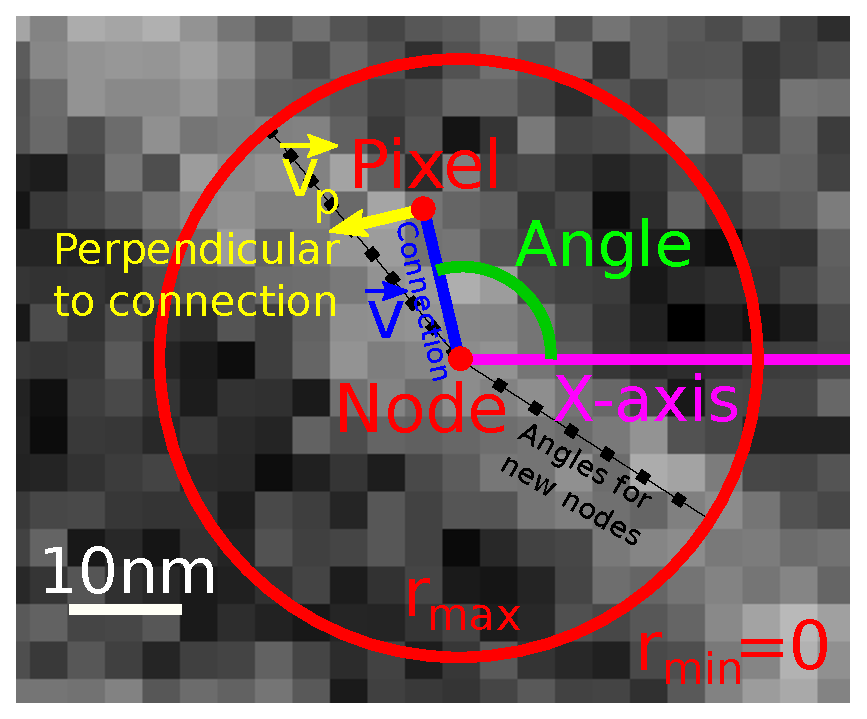
\includegraphics[width=\linewidth]{figures/tracking_illustration.eps}
	\caption{SEM image of an actin fiber imaged by Daniel Flormann and illustrations clarifying the function of the automated fiber tracing algorithm.\\
	For each pixel between $r_{min}$ and $r_{max}$ the negative normalized second order derivative along $\vec{v}_p$ is computed along with the angle of $\vec{v}$ to the x-axis. These values are then used to determine in which angles new nodes are spawned.}
	\label{fig:track_ill}
\end{figure}
For each pixel that is being processed, two values are computed. The angle of $\vec{v}$ relative to the x-axis (See figure \ref{fig:track_ill}) and the negative normalized directional second order derivative in the pixel along $\vec{v_p}$. Here the latter value is abbreviated to $res$. In the following, the computation of $res$ will be described.\\
Be 
\begin{align*}
    H &=
    \left(
    \begin{array}{rr}
        a & b \\
        b & c \\
    \end{array}
    \right)\\
    a &= \frac{d^{2}}{dx^{2}} \\
    b &= \frac{d^{2}}{dx \, dy} = \frac{d^{2}}{dy \, dx}\\
    c &= \frac{d^{2}}{dy^{2}}\\
\end{align*}
the Hessian matrix in the pixel and $a$, $b$ and $c$ its corresponding entries (See \ref{sec:Hessian}).
The value of $res$ amounts to
\begin{align*}
	res &= -\frac{\vec{v_p}^{\,\intercal} \ H \ \vec{v_p}}{\lvert \vec{v_p}\rvert ^2}
\end{align*}
Here, $\vec{v_p}^{\,\intercal} \ H \ \vec{v_p}$ yields the second order derivative in the pixel along $\vec{v_p}$. The denominator of $\lvert \vec{v_p}\rvert ^2$ compensates for the length of $\vec{v_p}$ and normalizes the derivative. The $-$ flips the sign of everything. Because we expect the presence of a fiber to yield a negative second order derivative with a big absolute (See \ref{sec:Hessian_usefulness}), flipping the sign allows us to search for a big positive value of $res$. To actually compute $res$, the values for the vector $\vec{v_p}$ and the matirx $H$ need to be inserted:
\begin{align*}
	res &= - \frac{
	\left(-\Delta y \; , \; \Delta x \right)
	\left(
	\begin{array}{rr}
    		a & b \\
	    b & c \\
	\end{array}
	\right)
	 \left(\begin{array}{r} -\Delta y \\ \Delta x \end{array} \right)
	 }{\Delta x ^2 + \Delta y ^2}\\
	& = - \frac{ \Delta y^2 \ a - 2 \ \Delta x \ \Delta y \ b + \Delta x ^2 \ c }{\Delta x ^2 + \Delta y ^2}
\end{align*}
Now for each of the selected pixels, two values have been computed. The angle of $\vec{v}$ to the x-axis and $res$. From now on, the angle of $\vec{v}$ to the x-axis is abbreviated to $ang$. This yields the ordered pair $(ang,res)$ for every processed pixel. The goal of the function described here is to find angles along which fibers travel. These will be the angles, where the corresponding $res$ values are predominantly big. Since $res$ values are only known for discrete $ang$ values, these $ang$ values are not equidistant and the $ang$ values of several pixels can even be identical, the individual $res$ values are not well suited to determine any such angles. Subsequently a way to find angles, where the $res$ values in the vicinity are generally large is required. Therefore a measure, that takes several $res$ values with similar $ang$ values into account is needed. To achieve this, a weighted average over the $res$ values is used. This weight is only significant for the $res$ values within a small angle interval. Specifically, the weight of the $res$ values is given by a Gaussian of the $ang$ values. This measure can be evaluated for any angle, by shifting the center of the Gaussian to that angle. The standard deviation $\sigma_{smooth}$ of this Gaussian has to be specified and can be used to control the size of the angle interval with significant weight. This measure evaluated at a specific angle $\alpha$ is abbreviated to $smooth(\alpha)$, because the resulting function can be regarded as a smoothing of the angle dependent $res$ values. It should be noted that this Gaussian wraps around, since the angle describes a closed circle (See figure \ref{subfig:smooth_weight1}).
\begin{figure}[h!]
	\begin{subfigure}[b]{\linewidth}
	    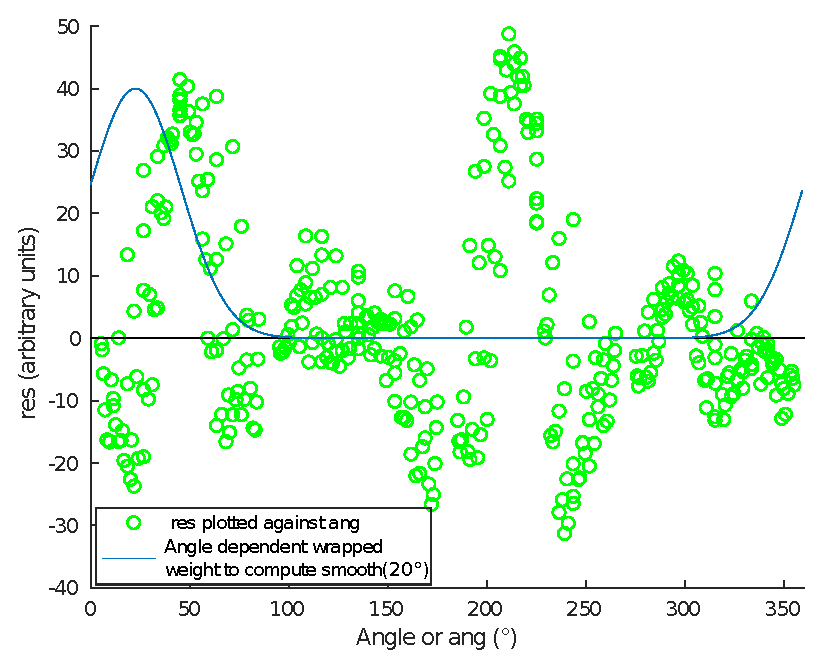
\includegraphics[width=\linewidth]{figures/ang_fun1.eps}
	    \caption{Visualization of the angle dependent weight for the $res$ values used to compute $smooth(\alpha)$.}
	    \label{subfig:smooth_weight1}
	\end{subfigure}
	\begin{subfigure}[b]{\linewidth}
	    \includegraphics[width=\linewidth]{figures/ang_fun2.eps}
	    \caption{The local maxima of $smooth(\alpha)$ are the angles in which new nodes are spawned if they lie above the threshold $thresh$ (Here $thresh = 0$)}
	    \label{subfig:smooth_weight2}
	\end{subfigure}
    \caption{Nodes spawn new nodes in the angles where $smooth(\alpha)$ has a local maximum above $thresh$ (See figure \ref{subfig:smooth_weight2}). $smooth(\alpha)$ is computed by the weighted mean of the $res$ values. This angle dependent weights is shown in figure \ref{subfig:smooth_weight1}. The $res$ values can be thought of as a negative angle dependent second order derivative.}
    \label{fig:smooth_weight}
\end{figure}
Mathematically $smooth(\alpha)$ is computed by
\begin{align*}
	weight_i &:= \ \exp{\left(\frac{(ang_i-\alpha)^2}{2 \ \sigma_{smooth}^2}\right)} \\
	& + \exp{\left(\frac{(ang_i-\alpha + 2 \pi)^2}{2 \ \sigma_{smooth}^2}\right)} \\
	& + \exp{\left(\frac{(ang_i-\alpha - 2 \pi)^2}{2 \ \sigma_{smooth}^2}\right)} \\
	smooth(\alpha) &= \ \frac{\sum_{i=1}^{n} res_i \ weight_i}{\sum_{i=1}^{n} weight_i}
\end{align*}
where $n$ is the total number of processed pixels, $res_i$ the $res$ value of the i-th computed pixel and $ang_i$ the $ang$ value of the i-th computed pixel. The two additional summands to the weight of the i-th computed pixel $weight_i$ are to wrap the Gaussian around the circle once. Theoretically a infinite amount of Gaussians would have to be summed up, each shifted by $2 \pi$, but the contributions of the missing terms are negligible in the usable $\sigma_{smooth}$ range (See \ref{sec:input_params}).\\
$smooth(\alpha)$ is then computed for a specifiable number of angles, that are evenly distributed between $0$ and $2 \pi$ radians (See figure \ref{fig:smooth_weight}). The number of points, $smooth(\alpha)$ is computed for, is a input parameter of the algorithm and called $steps$. Next the local maxima of the evaluated points of $smooth(\alpha)$ that lie above a specifiable threshold $thresh$ are determined. The angle of those local maxima are then used to try and spawn new nodes (See figure \ref{subfig:smooth_weight2}). The new nodes are spawned in those angles relative to the old node (See figure \ref{fig:track_ill}) in the specifiable distance $r_{step}$, when they lie inside the image and not to close to other already existing nodes.



\subsection{Preventing the crossing of connections}
To prevent connections between nodes from crossing each other, which would cause an oversampling, a minimal distance between the nodes was implemented. If a new node is to be placed closer to a existing node than $\frac{r_{step}}{\sqrt{2}}$, the node will not be placed (See figure \ref{fig:min_dist}).
\begin{figure}[h!]
	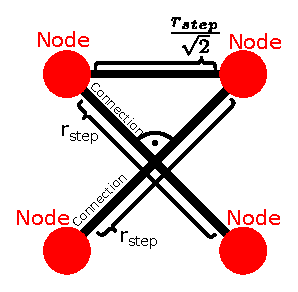
\includegraphics[width=\linewidth]{figures/min_dist.eps}
	\caption{The maximal distance between 4 node whose connections are crossed is $\frac{r_{step}}{\sqrt{2}}$}
	\label{fig:min_dist}
\end{figure}
\subsection{Connections between existing nodes} \label{sec:closures}
The part of the algorithm that has been described so far only allows for branching in the network. But there has to be a way for the branches to reunite and form closed loops. To achieve this, two already existing nodes can connect under certain conditions. This can happen, when a node A wants to spawn a new node that would be too close to an already existing node B. If this condition is met, it is checked whether these two nodes A and B are already connected in the network over a specifiable number of steps $min\_loop\_length$. More specifically, the check is if it is possible to jump only between connected nodes from node A within $min\_loop\_length$ steps to node B. If this is not possible, the two nodes are connected (See figure \ref{fig:min_loop_length}). If $min\_loop\_length$ is set to zero or this second check is not done, the algorithm will constantly build triangles and connect way too many nodes.
\begin{figure}[h!]
	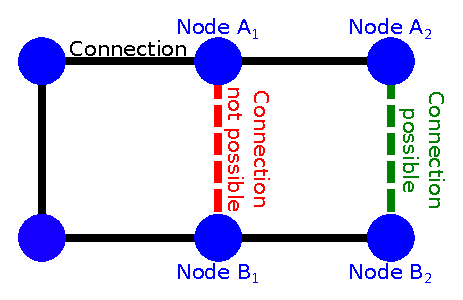
\includegraphics[width=\linewidth]{figures/min_loop_length.eps}
	\caption{Example of the effects of $min\_loop\_length$. Here $min\_loop\_length = 4$ therefore the left connection between the nodes A$_1$ and B$_1$ not possible but the one between A$_2$ and B$_2$ is.}
	\label{fig:min_loop_length}
\end{figure}



\subsection{Extracted parameters} \label{sec:extr_params}
The raw tracing data does not help directly when trying to find differences in images. Therefor relevant parameters have to be extracted from the tracing data to allow for useful quantification of the image.\\

One of the most relevant parameters in the context of actin meshes is the mesh hole size since it is assumed to correlate with the physical properties of the cell \cite{actin_gel_on_spherical_surface}. In the tracing data mesh holes are easily defined as closed loops inside of which there are no other closed loops. Their size can now be quantified by any number of measures such as their area or their circumference. Therefore once the meshwork has been traced accurately, the distribution of its mesh hole size can be extracted and compared between different conditions.\\

The tracing data also allows for the easy recognition of fiber junctions or branches. These junctions can easily be recognized by the nodes that are connected to more than two other nodes. In a continuous fiber without junctions each node is connected to exactly two other nodes while its endpoints are connected to only one other node. Therefor any node that has more than two connections is regarded as a junction of fibers. Now the distances between those junctions can be easily computed and regarded as a measure for fiber length or cross linking frequency of the network. This measure will, however, underestimate fiber length since not all fibers end at their junctions and therefore has to be used with caution.\\

%Another interesting quantification of the network would be the angle distribution of the fiber junctions, because some proteins like the Arp2/3 complex branch actin filaments at specific angles. To compute this angle distribution three methods have been implemented. The simplest is to calculate all relative angles of the connections of junctions. These angles exactly at the junctions are, however, often slightly skewed because the branching can only take place at the discrete nodes that do not usually lie in the exact center of the junction. Therefore a slightly more sophisticated method was implemented. This method starts at the nodes connected to the junction and then walks a specifiable number of nodes away from the junction. Next the direction from the node after these steps to the node connected to the junction is computed. This is done for all nodes that are connected to the junction and the relative angles between the resulting directions are saved. A third method uses the eigenvector of the smaller eigenvalue of the hessian. Here the pixels closest to the nodes that lie a specifiable number of steps distant to the junction are chosen. The correspondent hessian and the eigenvector is computed. Next the relative angles between all the resulting eigenvectors are saved. This method relies more on the image than on the tracing data.\\

%The\label{sec:extr_params_length} fiber length distribution would also be of interest. To find it, a function was implemented that walks along the network, always choosing the straightest connection between nodes. If there is no connection within a specifiable angle interval, so that there is a sufficiently big kink in the tracing data, the function assumes the fiber to stop. Here all nodes that are not junctions can only belong to one single fiber. Now, upon other parameters, the length of the fibers that were determined this way can be computed.\\




\section{Validation of the tracing algorithm}
%Since there is no ground truth for our SEM images, we can only perform some tests on our fiber tracing algorithm to estimate its performance and find its breaking points.
\subsection{Highest reliably traceable fiber density}
A test was performed to find the highest reliably traceable fiber density. For this test, artificial images were created. These were 1000 by 1000 pixels in size and a grid of horizontal and vertical white lines five pixel in thickness was generated on a black background. As a measure for line density, the percentage of black pixels on the image was used since black pixels are not part of any line. When the amount of white lines increases, the percentage of black pixels on the image decreases. The images were traced with parameters that also worked well on SEM images of the actin cortex of adherent cells (See table \ref{tab:parameters_dense}). As a measure for the quality of the fiber tracing, the mesh hole areas computed by the algorithm were compared to the known mesh hole areas of the generated image (See figure \ref{fig:dev_linedense}). This discrepancy between the exact and computed values was then expressed by the standard deviation of the computed areas from the exact areas. Be $a_{exact}$ the exact mesh hole area of the generated image and be $a_{comp_{i}}$ the i-th computed mesh hole area. Furthermore be $n$ the number of computed areas. Then the standard deviation $dev$ of the computed areas from the exact value is:
\begin{align*}
	dev = \sqrt{\sum_{i=1}^n \frac{(a_{comp_{i}} - a_{exact})^2}{n}}
\end{align*}
This standard deviation $dev$ was expressed as a percentage of the exact value and mapped to the percentage of black pixels in figure \ref{subfig:dev_percent}. In figure \ref{fig:dev_linedense} a big increase in the discrepancy between the computed and exact values can be observed below the 20\% black pixel mark. The image with the highest still reasonably well tractable fiber density is shown in figure \ref{fig:last_working}.
\begin{figure}[h!]
	\begin{subfigure}[b]{\linewidth}
		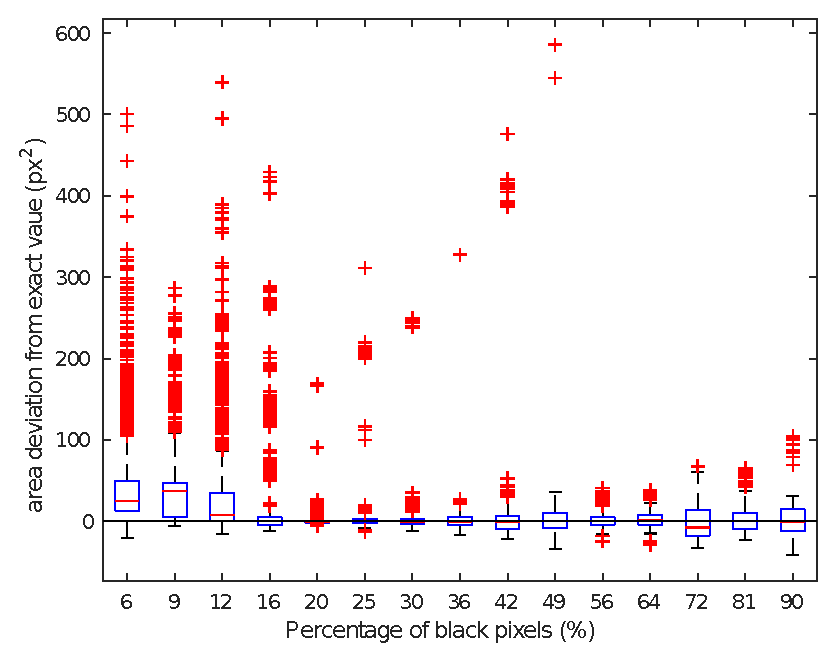
\includegraphics[width=\linewidth]{illustrations/line_density_new_1.eps}
		\caption{The deviation of the computed areas from the exact value mapped to the percentage of black pixels. Ideally all data points should lie on the x-axis.}
		\label{subfig:dev_boxplot}
	\end{subfigure}
	\begin{subfigure}[b]{\linewidth}
		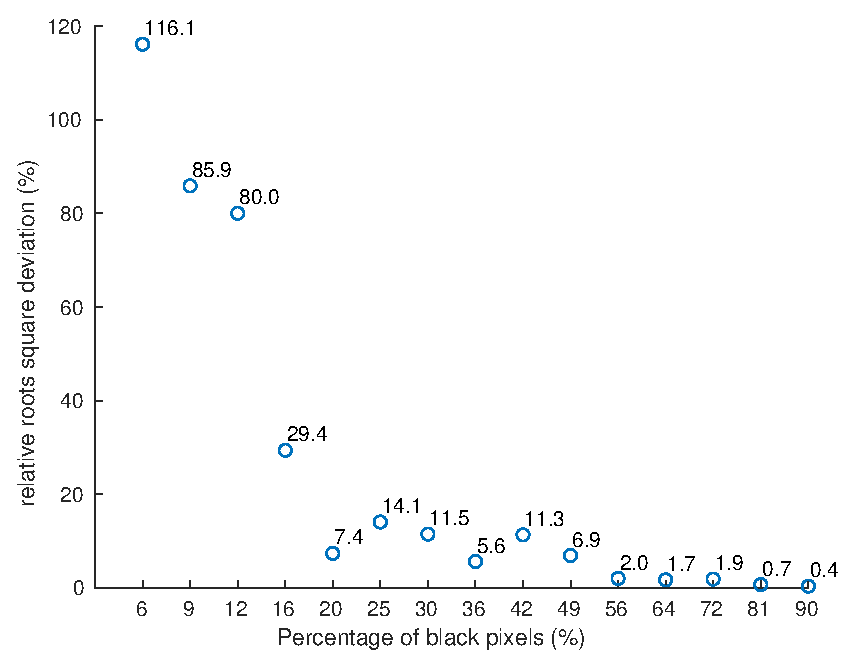
\includegraphics[width=\linewidth]{illustrations/line_density_new_2.eps}
		\caption{Standard deviation of the computed areas from the exact value expressed as a percentage of the exact value mapped to the percentage of black pixels.}
		\label{subfig:dev_percent}
	\end{subfigure}
	\caption{Test for the highest reliably traceable fiber density by comparing the known mesh hole areas of generated images to the mesh hole area distribution computed by the tracing. The images were generated as white lines on a black background. Therefore the percentage of black pixels decreases as line density increases.}
	\label{fig:dev_linedense}
\end{figure}
\begin{figure}[h]
	\includegraphics[width=\linewidth]{illustrations/last_working.png}
	\caption{Generated image with the highest still reasonably well tractable fiber density.}
	\label{fig:last_working}
\end{figure}
\begin{table}[h!]
\centering
\caption{Parameter set used to trace the generated images with varying fiber density.}
\label{tab:parameters_dense}
\begin{tabular}{c|c}
	Parameter & Value\\
	\hline
	$\sigma_{conv}$ & 2.3 pixel\\
	$r_{min}$ & 0 pixel\\
	$r_{max}$ & 8 pixel\\
	$\sigma_{smooth}$ & 0.55 radians\\
	$steps$ & 360\\
	$thresh$ & 0.5\\
	$r_{step}$ & 3 pixel\\
	$min\_loop\_length$ & 7\\
\end{tabular}
\end{table}
Therefore we can expect the algorithm to not be drastically affected by fiber density if no more than 80\% of the pixels in a image are part of fibers. Also the parameters were not optimized for the generated images, so when the parameters of the tracing algorithm are adjusted, even higher line densities could likely be traced reliably.


\subsection{Validation of mesh hole areas on images with known ground truth}
A already existing fiber quantification tool is DiameterJ \cite{diaj}. It is a plugin for ImageJ \cite{imj}. For the validation and of this plugin, a dataset was published \cite{diaj_dataset} from which 3 suitable images were selected. One of these images is shown in figure \ref{fig:diaj_traced}. They were selected, because they are already segmented into only black and white pixels and therefore the output of DiameterJ can be regarded as ground truth. Also the images did not consist of regular patterns, making the tracing more difficult and likely to fail. Additionally the white lines were 3 pixel thick, a value comparable to the thickness of actin fibers in our SEM images. DiameterJ considers the thickness of the fibers when computing the mesh hole areas. To account for this, the circumference times half the fiber diameter was subtracted from the area of every loop in the tracing data. The tracing was done using a parameterset that also works well on the SEM images of the actin fibers (See table \ref{tab:parameters_diaj}) our program was developed for. The mean values computed from the DiameterJ mesh hole area distributions were never more than 10\% off from the values our tracing algorithm produced. Also the mean produced by DiameterJ is always between 6\% and 10\% more than our result. Therefore all our results deviate in a similar way from the ground, causing the results to be very comparable (See figure \ref{fig:diaj_comp}).
\begin{figure}[h!]
	\begin{subfigure}[b]{\linewidth}
		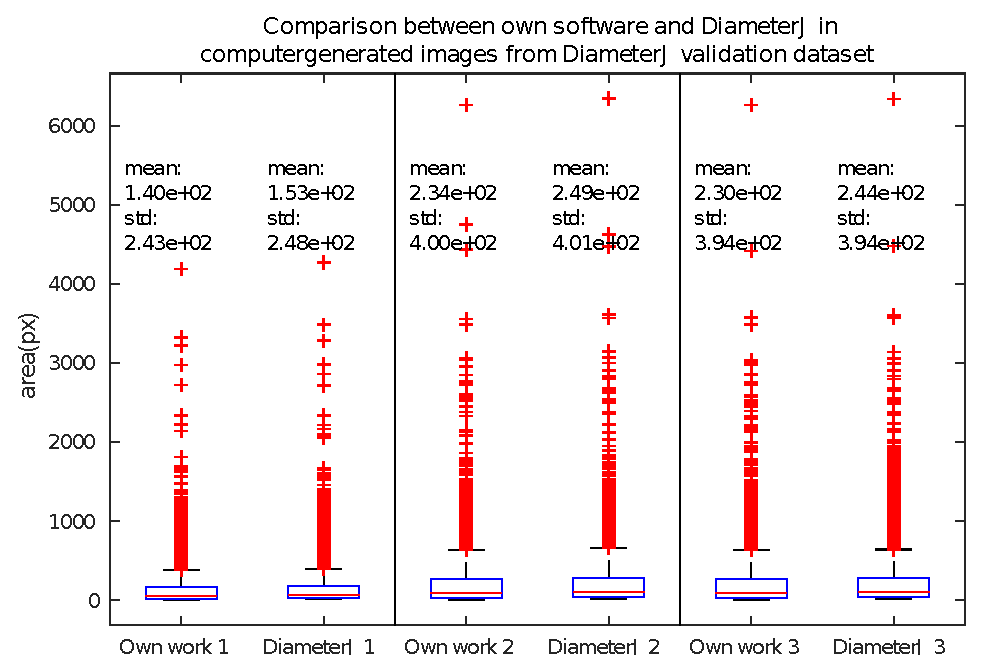
\includegraphics[width=\linewidth]{illustrations/sef_vs_diaj_new.eps}
		\caption{Mesh hole area distributions produced by DiameterJ and our fiber tracing algorithm.}
		\label{subfig:self_vs_diaj}
	\end{subfigure}
	\begin{subfigure}[b]{\linewidth}
		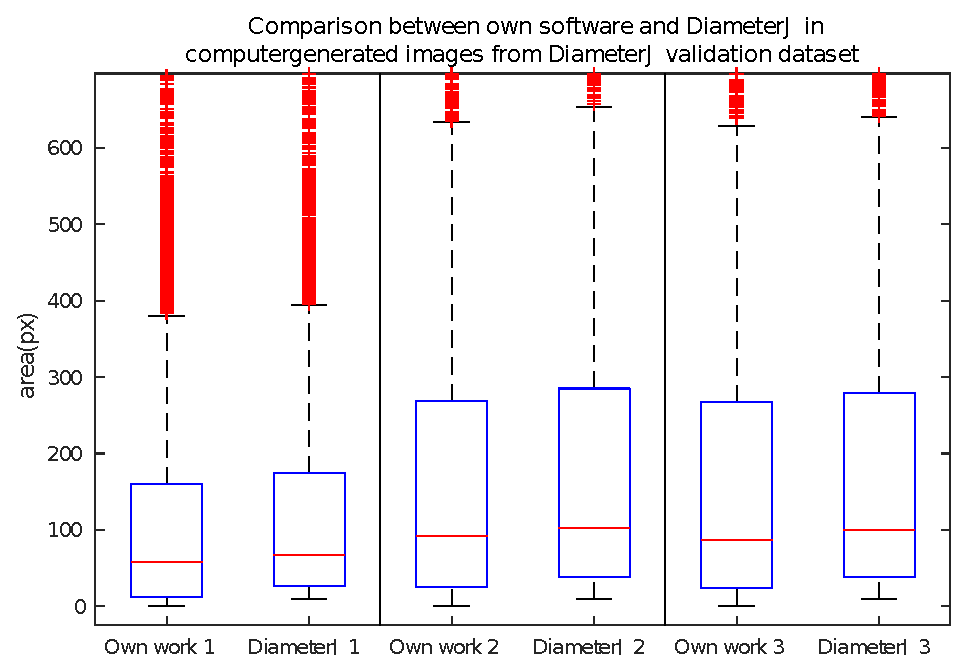
\includegraphics[width=\linewidth]{illustrations/sef_vs_diaj_new_zoom.eps}
		\caption{Figure \ref{subfig:self_vs_diaj} magnified}
	\end{subfigure}
	\caption{Evaluating the viability of our fiber tracing algorithm by comparing the produced mesh hole area distribution to the one generated by DiameterJ. The images analyzed for this test only consisted of black and white pixels (See figure \ref{fig:diaj_traced}) and therefore the output of DiameterJ can be regarded as ground truth.}
	\label{fig:diaj_comp}
\end{figure}
\begin{figure*}[t]
	\includegraphics[width=\linewidth]{illustrations/diaj_traced.png}
	\caption{Image from the DiameterJ validation dataset \cite{diaj_dataset} with visualized tracing data from our fiber tracing algorithm. The original image from the dataset is only black and white, all colored lines are part of the visualized tracing data. Blue lines are part of a closed loop and green lines are not and therefore green lines do not contribute to the mesh hole area distribution.}
	\label{fig:diaj_traced}
\end{figure*}
\begin{table}[h!]
\centering
\caption{Parameter set used to trace the images from the DiameterJ validation dataset \cite{diaj_dataset}.}
\label{tab:parameters_diaj}
\begin{tabular}{c|c}
	Parameter & Value\\
	\hline
	$\sigma_{conv}$ & 1.8 pixel\\
	$r_{min}$ & 0 pixel\\
	$r_{max}$ & 8 pixel\\
	$\sigma_{smooth}$ & 0.55 radians\\
	$steps$ & 360\\
	$thresh$ & 0.5\\
	$r_{step}$ & 3 pixel\\
	$min\_loop\_length$ & 7\\
\end{tabular}
\end{table}


\subsection{Comparison to DiamerJ on our SEM images of the actin cortex}
DiameterJ is a easily accessible fiber analysis software that can extract some of the parameters we are interested in, such as the mesh hole area distribution. When it is applied to our specific imaging results of the actin cortex, many fibers are not found (See figure \ref{fig:our_vs_diaj_og}). Our software shows superior fiber recognition on these specific images. While it can also be argued, that the analysis by DiameterJ can be used to objectively compare different conditions and the imperfections cancel out in the comparison, starting with a more representative analysis will ensure better comparability.
\begin{figure}[h]
    \centering
    \begin{subfigure}[b]{\linewidth}
        \includegraphics[width=.9\linewidth]{figures/new_trace_og.png}
        \caption{SEM image of actin cortex with visualized tracing data from our program. Blue lines are not part of any closed loop and do therefore not contribute to the mesh hole area distribution, in contrast to the red lines. Parameters used for tracing in table \ref{tab:parameters}}
        \label{subfig:our_traced_og}
    \end{subfigure}
    \begin{subfigure}[b]{\linewidth}
        \includegraphics[width=.9\linewidth]{illustrations/og_diaj2.png}
        \caption{Fibers found on image \ref{subfig:our_traced_og} by DiameterJ.}
    \end{subfigure}
    \caption{Comparison between the fibers found by our software and DiameterJ on a SEM images of the actin cortex. Imaging by Daniel Flormann.}
    \label{fig:our_vs_diaj_og}
\end{figure}
\subsection{Advantages and limitations of our analysis}
As is visible in figure \ref{subfig:our_traced_og}, most fibers are traced accurately. There are, however, some fibers that are not recognized and some traces that do not correspond to any fiber. Also the three-dimensional structure of the network is not taken into account at all. But it is unlikely, that any fiber recognition software will ever yield perfect results on these images, due to the present noise, limited resolution and impurities on the sample. Additionally because the obtained images are only two-dimensional, we are not able to resolve the three-dimensional structure of the actin network. Also manual fiber tracing is unlikely to yield repeatable results for different operators because some structures can not be explicitly identified. The results of our software on the other hand are repeatable, and the imperfections in the tracing data are present in all analyzed images to the same degree. Therefore the parameters extracted from the tracing of different images can be compared and used to objectively quantify the differences between conditions. Furthermore the large amount of data generated by the tracing of each image ensures good statistics, comparability and causes random variations to be less significant. In each analyzed image, several hundred up to thousands of mesh holes are found.
\begin{table}[h!] \label{tab:parameters}
\centering
\caption{Parameter set used to trace all SEM images that were analyzed for this work.}
\label{tab:parameters}
\begin{tabular}{c|c}
	Parameter & Value\\
	\hline
	$\sigma_{conv}$ & 1.8 pixel\\
	$r_{min}$ & 0 pixel\\
	$r_{max}$ & 8 pixel\\
	$\sigma_{smooth}$ & 0.5 radians\\
	$steps$ & 360\\
	$thresh$ & 2\\
	$r_{step}$ & 3 pixel\\
	$min\_loop\_length$ & 7\\
\end{tabular}
\end{table}

\section{Mathematical background}
\subsection{Mathematical operations on images}
\subsubsection{Derivatives and convolutions of images} \label{sec:how_to_derive_images}
Images can be understood as functions, that map a two-dimensional space to a one-dimensional space. Specifically, the pixel-position is mapped to the pixel brightness. Of course, this map is only defined at discrete points namely the pixels but can be approximated as a continuous map. Here it should be noted, that these maps that correspond to the images can be thought of as bounded and arbitrarily smooth. This is the case, because the values of images are bounded and are only defined at discrete points (pixels) with finitely small distances between them. Therefore the map corresponding to the image can be interpolated between the pixels in a arbitrarily smooth way. Therefore not only the image its self is bounded but all derivatives as well. This approximation of images as continuous maps allows us to apply mathematical operations to the image to enhance or get rid of certain features. Specifically, we can compute the derivatives of the map corresponding to the image. If we compute the derivative directly on the original image, any noise will be strongly amplified by the derivative, making the output unusable. Therefore the image usually has to be smoothed for noise reduction first. This is especially true for SEM images since they are prone to noise. This noise reduction or smoothing can be achieved by convoluting the image with a Gaussian kernel. Mathematically the convolution of a map $f(\Vec{r})$ with a kernel $k(\Vec{r})$ is defined as:\\
\begin{align*}
    (f * k)(\Vec{r}) = \int f(\Vec{r'}) \ k(\Vec{r'} + \Vec{r}) \ d\Vec{r'}
\end{align*}
The Gaussian kernel $g(\Vec{r})$ is defined as:
\begin{align*}
    g(\Vec{r}) = \frac{1}{\sigma \, \sqrt{2 \, \pi}} \, \exp{-\frac{\Vec{r\,}^2}{2 \, \sigma}}
\end{align*}
With the standard deviation $\sigma$ and the position vector $\Vec{r}$. In practice on an image, the kernel also consists of discrete pixels and is usually smaller than the picture. The kernel is scanned over the image, while the kernel pixel values are multiplied with the corresponding image pixel values to compute the convoluted image.\\
This way the picture can be smoothed and the noise drastically reduced. But the derivatives still have to be computed. This is difficult on a discrete map because the derivative of a function $f(\Vec{r})$ in the direction $\Vec{u}$ is defined as $\frac{df(\Vec{r})}{d\Vec{u}} = \lim_{h\to 0}\frac{f(\Vec{r}+h \, \Vec{u}) - f(\Vec{r})}{h}$, but the pixels have discrete distances and therefore the $\lim_{h\to0}$ can not be computed with arbitrary precision.\\
Instead of first smoothing the image and then computing the derivatives, both those steps can be combined into one. To illustrate this, let us consider the derivative of a  convolution of sufficiently smooth function $f(\Vec{r})$ and kernel $k(\Vec{r})$: \\
\begin{align*}
    &\frac{d}{d r_{i}}(f * k)(\Vec{r})\\
    &= \frac{d}{d r_{i}} \int f(\Vec{r'}) \ k(\Vec{r'} + \Vec{r}) \ d\Vec{r'}\\
    &= \int f(\Vec{r'}) \  \frac{d}{d r_{i}}k(\Vec{r'} + \Vec{r}) \ d\Vec{r'}\\
    &= \int f(\Vec{r'}) \ k_{i}(\Vec{r'} + \Vec{r}) \ d\Vec{r'}
\end{align*}
Where $r_{i}$ is the i-th coordinate and $k_{i}(\Vec{r})$ is the derivative in the i- th coordinate of the kernel. So instead of first convoluting and then calculating the derivative, we can simply convolute with the derivative of the kernel $k(\Vec{r})$. This is especially useful if the discrete kernel for picture convolution is generated by discrete evaluations of a analytical function like the Gaussian kernel. This way we can calculate the analytical derivative for maximal accuracy before the discrete evaluation of the kernel.\\
With this method we can compute any order derivative by simply deriving the kernel.

\subsubsection{The Hessian matrix of images} \label{sec:Hessian}
Image brightness profile curvature can be used to enhance the visibility of fibers in an image (See \ref{sec:Hessian_usefulness}). The second-order derivative or curvature of a two dimensional map $f:\mathds{R}^{2}\to \mathds{R}; \ (x,y) \mapsto f(x,y)$ takes the form of a 2x2-Matrix called the Hessian matrix $H$: \\
\begin{align*}
 H = 
    \left(
    \begin{array}{rr}
        \frac{d^{2}f}{dx^{2}} & \frac{d^{2}f}{dx \, dy} \\
        \frac{d^{2}f}{dy \, dx} & \frac{d^{2}f}{dy^{2}} \\
    \end{array}
    \right)
\end{align*}
Here, $\frac{d^{2}}{dx \, dy} = \frac{d^{2}}{dy \, dx}$ holds for sufficiently smooth functions due to the theorem of Schwarz. Therefore the Hessian matrix is symmetric and we obtain 3 different analytical kernels or derivatives of the Gaussian $g(x,y)$. To calculate the Hessian in every pixel of the smoothed image, we convolute the image with the 3 discrete kernels obtained by evaluating the analytical derivatives of the Gaussian $g(x,y) = \frac{1}{\sigma \, \sqrt{2 \, \pi}} \, \exp{-\frac{x^2 + y^2}{2 \, \sigma}}$(See Figure \ref{fig:Hessian_kernels}).
\begin{align*}
    &\frac{d^{2}}{dx^{2}} \, g = \frac{\left( \left(\frac{x}{\sigma} \right)^{2} - 1\right)\exp{-\frac{x^{2} + y^{2}}{2 \, \sigma^{2}}}}{\sigma^{3} \sqrt{2 \, \pi}} \\
    &\frac{d^{2}}{dx \, dy} \, g = \frac{d^{2}}{dy \, dx} \, g = \frac{x \, y \, \exp{-\frac{x^{2} + y^{2}}{2 \, \sigma^{2}}}}{\sigma^{5} \sqrt{2 \, \pi}}  \\
    &\frac{d^{2}}{dx^{2}} \, g = \frac{\left( \left(\frac{y}{\sigma} \right)^{2} - 1\right)\exp{-\frac{x^{2} + y^{2}}{2 \, \sigma^{2}}}}{\sigma^{3} \sqrt{2 \, \pi}}  \\
\end{align*}
\begin{figure}[h]
    \centering
    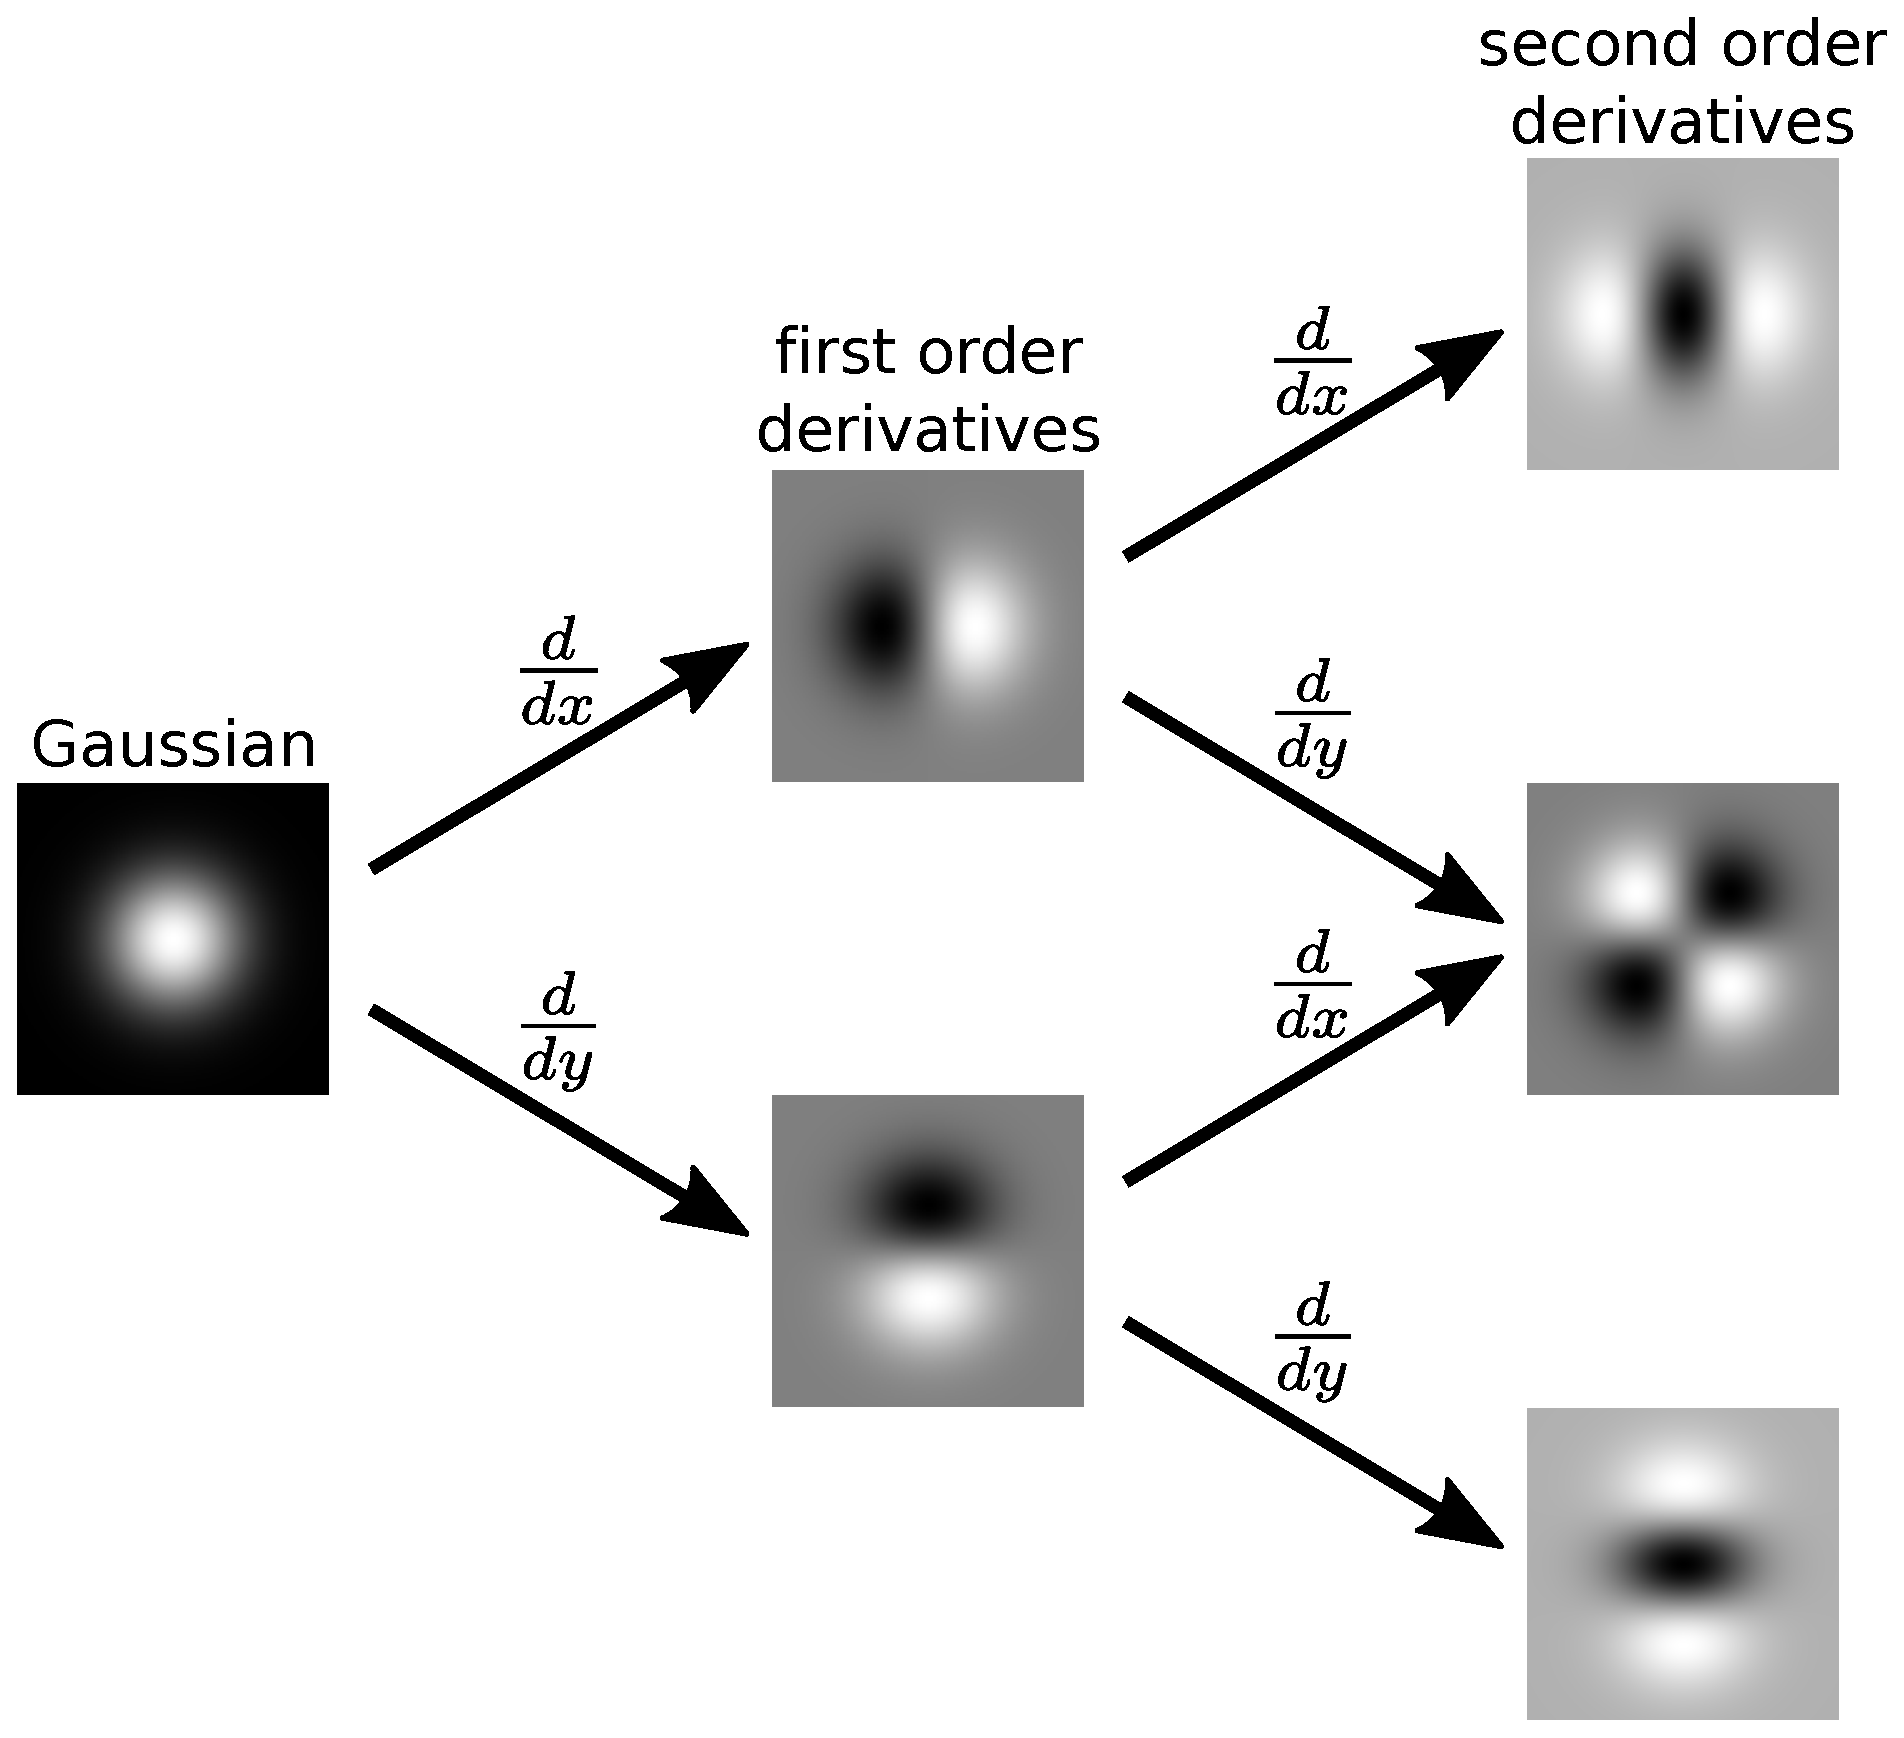
\includegraphics[width=.9\linewidth]{illustrations/gaussian_derivatives.eps}
    \caption{Visualization of the discrete kernels obtained by evaluation of the analytical derivatives of the Gaussian.\\
    		Visualization generated by OpenCV  \cite{opencv_library}}
    \label{fig:Hessian_kernels}
\end{figure}
If we choose to look at the curvature of a specific point or pixel with coordinates $(x,y)$ the Hessian $H$ takes the form:
\begin{align*}
    H &=
    \left(
    \begin{array}{rr}
        a & b \\
        b & c \\
    \end{array}
    \right)\\
    a &= \frac{d^{2}f(x,y)}{dx^{2}} \\
    b &= \frac{d^{2}f(x,y)}{dx \, dy} = \frac{d^{2}f(x,y)}{dy \, dx}\\
    c &= \frac{d^{2}f(x,y)}{dy^{2}}\\
\end{align*}
Using this Hessian matrix $H$ any second-order directional derivatives in this point can easily be computed as:
\begin{align*}
    \frac{d^2f(\Vec{r})}{d\Vec{u}^{\,2}} &=\Vec{u}^{\,\intercal} H \Vec{u} = a\,u_x^2 + 2\,b\,u_x\,u_y + c\,u_y^2 \\
    \Vec{u} &= \left(
    \begin{array}{c}
        u_x\\
        u_y
    \end{array}
    \right); \ \Vec{r} = \left(
    \begin{array}{c}
        x\\
        y
    \end{array} \right)
\end{align*}
Here it should be noted, that this second order directional derivative scales with $|\Vec{u}|^2$. Therefore we implicitly assume, that $|\Vec{u}| = 1$ when comparing directional derivatives from here on.\\
To better understand the information contained in the Hessian matrix, we can work out the eigenvalues:
\begin{align*}
    \lambda_1 = \frac{a + c - \sqrt{(a - c)^2 + 4\,b^2}}{2}\\
    \lambda_2 = \frac{a + c + \sqrt{(a - c)^2 + 4\,b^2}}{2}
\end{align*}
and the two perpendicular not normalized eigenvectors:
\begin{align*}
    \Vec{v_1} &= \left(
    \begin{array}{c}
         a - c - \sqrt{(a - c)^2 + 4\,b^2}\\
         2\,b
    \end{array}
    \right)\\
    &= 2\,\left(
    \begin{array}{c}
         \lambda_1 - c\\
         b
    \end{array}
    \right)
    \\
    \Vec{v_2} &= \left(
    \begin{array}{c}
         a - c + \sqrt{(a - c)^2 + 4\,b^2}\\
         2\,b
    \end{array}
    \right)\\
    &= 2\,\left(
    \begin{array}{c}
         \lambda_2 - c\\
         b
    \end{array}
    \right)
\end{align*}
Here $\lambda_1$ is the smallest possible second-order directional derivative and $\Vec{v_1}$ indicates the associated direction of smallest curvature. Conversely $\lambda_2$ is the biggest curvature value and $\Vec{v_2}$ the associated direction. This is because $\sqrt{(a - c)^2 + 4\,b^2} > 0$ and the only difference between $\lambda_1$ and $\lambda_2$ is the sign before this summand.\\
Here it is important to note that this statement does not apply to the absolute values of $\lambda_1$ and $\lambda_2$ since they can both either be positive or negative. Therefore the function might be much more strongly curved in the direction of $\Vec{v_1}$ than in the direction of $\Vec{v_2}$ because $\Vec{v_1}$ has a large absolute value and is negative.\\
If we do a coordinate transform and use the normalized versions of $v_1$ and $v_2$ as basis vectors, the Hessian matrix becomes the diagonal matrix:
\begin{align*}
    H =
    \left(
    \begin{array}{cc}
        \lambda_{1} & 0 \\
        0 & \lambda_{2} \\
    \end{array}
    \right)
\end{align*}
meaning, that in this new coordinate system, the mixed derivative terms are not important ($\frac{d^{2}}{dx \, dy} = \frac{d^{2}}{dy \, dx} = 0$).


\subsubsection{Usefulness of the Hessian matrix in fiber recognition} \label{sec:Hessian_usefulness}
\begin{figure}[h]
    \centering
    \begin{subfigure}[b]{\linewidth}
        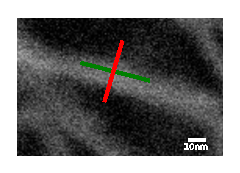
\includegraphics[width=.9\linewidth]{figures/curvatur_real_fibre.eps}
        \caption{SEM image of actin fiber. Imaged by Daniel Flormann.}
        \label{subfig:profile_img}
    \end{subfigure}
    \begin{subfigure}[b]{\linewidth}
        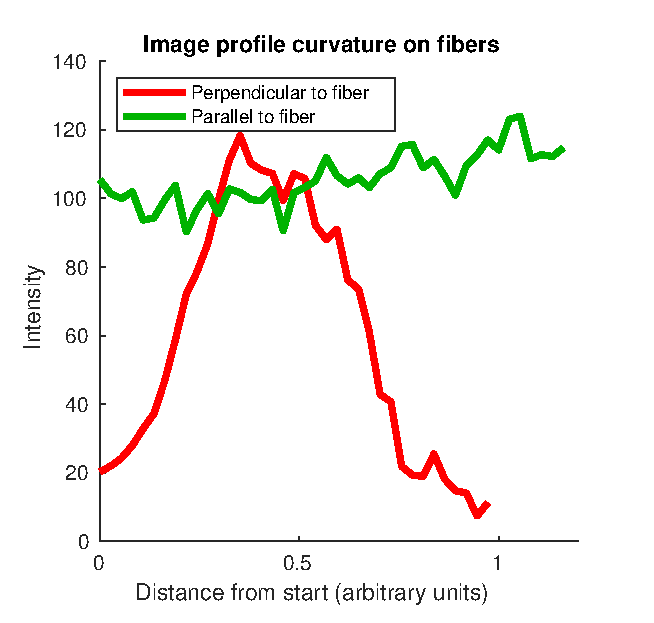
\includegraphics[width=.9\linewidth]{figures/curvature2.eps}
        \caption{image brightness profile of lines drawn in figure \ref{subfig:profile_img}.\\
        Intensity profile generated by Fiji \cite{fiji}.}
    \end{subfigure}
    \caption{When travelling along a fiber, the image brightness profile is relatively constant and when travelling perpendicular to a fiber, the image brightness forms a local maximum in the middle of the fiber. This causes a large negative second-order derivative or curvature in the middle of fibers.}
    \label{fig:curvature_example}
\end{figure}
\begin{figure}[h!]
    \centering
    \begin{subfigure}[b]{\linewidth}
        \includegraphics[width=.85\linewidth]{figures/og_image.png}
        \caption{SEM image of actin fibers by Daniel Flormann.}
        \label{subfig:og1}
    \end{subfigure}
    \begin{subfigure}[b]{\linewidth}
        \includegraphics[width=.85\linewidth]{figures/viz.png}
        \caption{$-1$ times smaller eigenvalue of the Hessian matrix of figure \ref{subfig:og1} is mapped to the brightness. The color encodes the direction of the corresponding eigenvector. This causes fibers travelling in the same direction have the same color. (See \ref{sec:how_to_derive_images} and \ref{sec:Hessian})}
        \label{subfig:-lambda1}
    \end{subfigure}
    \caption{Using the eigenvalues of the Hessian to remove noise and background and enhance fiber visibility. The Hessian is computed by calculating the second order derivatives of the Gaussian filter. Then the smaller eigenvalue is computed and its sign is flipped. The value obtained this way is displayed in figure \ref{subfig:-lambda1}.}
    \label{fig:-lambda1_vs_og}
\end{figure}
Fibers in images can be recognized as line like structures, whose brightness is different from the local background. Without loss of generality, here we assume them to be brighter than the local background.\\

Let us now consider a point in the middle of a fiber. The brightness of the image along the fiber is going to remain relatively constant. On the other hand, the brightness perpendicular to the fiber will decrease quickly, forward as well as backward. This means there is a local maximum of brightness in the middle of the fiber when looking at the image brightness on a line perpendicular to the fiber (See Figure \ref{fig:curvature_example}).  On a local maximum of a sufficiently smooth function, the second-order derivative or curvature is always negative.\\


For this reason, we expect the centres of fibers to have negative second order derivatives. We can use this for example to enhance the visibility of fibers in images and filter their the background. This can be archived by creating a new image, whose pixel values consist of $-1$ times the smaller eigenvalue of the Hessian matrix in that pixel (See figure \ref{fig:-lambda1_vs_og_1}). The $-1$ has to be used to swap the sign because we expect the second-order derivative to be negative on top of fibers. Also the eigenvector corresponding to this will be perpendicular to the fiber direction. Therefore we know the direction the fiber is travelling in (See figure \ref{fig:-lambda1_vs_og}). This method is very similar to the one used by Kikinis et. al. and was inspired by them \cite{tubeness_paper}. Another reason this second order derivative is useful for fiber recognition is, that the kernels used to compute the Hessian, can be thought of as a negative fiber template. They are dark in the middle, with two bright spots to the sides. Therefore, if such a kernel is placed on a fiber, that is bright with less brightness to its sides, it will yield a negative response with a large absolute value. If we now reverse the sign of this response, we obtain a map with enhanced fibers (See Figure \ref{fig:Hessian_kernels}).
\subsubsection{Using polar coordinates for fiber tracing} \label{sec:polar}
Usually, pixel positions of an image are expressed as Cartesian coordinates $(x,y)$. The value $x$ can be thought of as how far the pixel is to the right and $y$ as how far up the pixel is positioned. Therefore this coordinate system expresses position relative to two predefined directions, namely the basis vectors. The polar coordinates, on the other hand, use the angle $\phi$ and the radius $r$ to express position. Here $x = r \, \cos{\phi}$ and $y = r \, \sin{\phi}$. These coordinates have therefore no predefined directions or angles because the angle itself is a variable. For this reason, they are well suited for fiber tracking. If the origin of the polar coordinates is set on top of a fiber or line, bright pixels will accumulate at the angle, the line is travelling in (See figure \ref{fig:polar_parameterization}).  \cite{victor_small}

\begin{figure}[h]
    \centering
    \begin{subfigure}[b]{\linewidth}
        \includegraphics[width=.4\linewidth]{figures/polar_example.png}
        \caption{Example image in Cartesian coordinates}
        \label{subfig:cartesian}
    \end{subfigure}
    \begin{subfigure}[b]{\linewidth}
        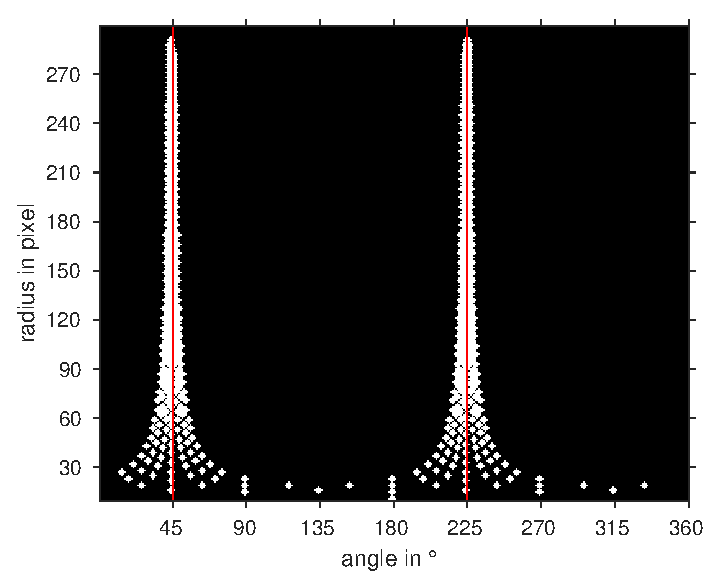
\includegraphics[width=\linewidth]{figures/polar_viz.eps}
        \caption{Figure \ref{subfig:cartesian} in polar coordinates. Origin of the polar coordinates is in the center of the image \ref{subfig:cartesian}}
        \label{subfig:polar}
    \end{subfigure}%
    \caption{Difference in parameterization of an image. Figure \ref{subfig:cartesian} shows the image in Cartesian coordinates and figure \ref{subfig:polar} shows all white pixels of figure \ref{subfig:cartesian} mapped to polar coordinates. The origin of the polar coordinates is in the middle of the figure \ref{subfig:cartesian}. Using figure \ref{subfig:polar} the angle, the line in \ref{subfig:cartesian} is traveling in, can easily be determined as 45\degree. This is indicated by the red vertical lines.\\
       Images generated using OpenCV  \cite{opencv_library}}
    \label{fig:polar_parameterization}
\end{figure}

%\afterpage{\clearpage}

%\lipsum

%\section{Analyzing our SEM images with DiameterJ}
%\begin{figure}[h!]
%    \centering
%    \begin{subfigure}[b]{\linewidth}
%        \includegraphics[width=\linewidth]{figures/og_image.png}
%        \caption{SEM image of actin fibers}
%    \end{subfigure}
%    \begin{subfigure}[b]{\linewidth}
%        \includegraphics[width=\linewidth]{figures/og_diaj2.png}
%        \caption{Fibers recognized by DiameterJ \cite{diaj}. Many fibers are not found making any data generated this way questionable.}
%    \end{subfigure}
%    \caption{Using the eigenvalues of the Hessian to remove noise and background and enhance fiber visibility. The Hessian is computed by calculating the second order derivatives of the Gaussian filter. Then the smaller eigenvalue is computed and its sign is flipped. The value obtained this way is displayed in figure \ref{subfig:-lambda1}.}
%    \label{fig:diaj_schlecht}
%\end{figure}
%When DiameterJ \cite{diaj} is applied directly to the images described in \ref{sec:our_images}, a lot of fibers are not recognized and therefore the extracted parameters are questionable. However, if DiameterJ  is applied to the images generated by $-1$ times the smaller eigenvalue of the Hessian matrix in each pixel, a lot more fibers are found and therefore the generated data would be a lot more reliable.

\subsection{Previous versions of the fiber tracing algorithm}
A developement history of the algorithm can be found at: \begin{verbatim}https://github.com/SRaent/Actin \end{verbatim}
Earlier versions only differ in one important part, namely the way nodes spawn new nodes (See \ref{sec:procreate}). The main difference here was, that instead of looking at the second order derivative of the image, the image brightness was used directly. Therefore the explanation given in \ref{sec:algo} still applies for all other parts. The section \ref{sec:procreate} is also still almost completely applicable, but instead of the $res$ value that is computed for every processed pixel, the pixel brightness was used and there was no threshold applied to the local maxima of the $smooth(\alpha)$ function, instead all local maxima were used to spawn new nodes. In this development stage the tracing algorithm was only slightly modified and the effort was focused on preprocessing the image to increase fiber visibility before applying the tracing algorithm. The first idea that was pursued in the hopes of increasing fiber visibility was to Fourier transform the image, apply a mask to the result and then perform the inverse Fourier transform. In the Fourier transform of a image, the information about the features of the image can be thought of as being ordered by the feature size. Since all fiber in our SEM image have the same thickness, the hope was, that the information about the fibers was mostly stored in a small part of the Fourier transform. After some experimentation, the best working mask for the Fourier transform was determined to be a hollow oval outside of which all frequency components were set to zero. A oval was necessary to select the same frequency components in all directions of a non square image. In the case of a square image with a aspect ration of 1:1, the oval would become a circle. The center of the oval was chosen at a frequency of 0.5 per fiber diameter, corresponding to a period of twice the fiber diameter (fiber diameter is about 4 pixel). The thickness of this oval then selects the frequency range around this center, that was used to generate the processed image. The thickness of the oval in the frequency space was chosen around half its semi major axis. Subsequently a small gaussian filter with a standard deviation of 1 pixel was applied to the image to reduce the left over noise. Next a threshold was applied to the pixel brightness. The brightness of pixels lying below that threshold were raised to that threshold. In the final step of image preprocessing, the brightness of the pixels was rescaled, so that the brightest pixel had a value of 255 and the darkest one a value of 0. This in combination with the previous threshold, set every pixel below the threshold to zero, since the darkest pixels in the image were the ones set to the threshold. All these steps led to a resulting image with reduced the noise, also caused by setting the contributions of high frequencies to zero and lower frequency contribution were also removed. In total, fiber visibility was somewhat increased. One big problem was, that the centers of larger mesh holes became almost as bright as the centers of the fibers. The biggest problem during this phase of the development was however that the fiber tracing would very often connect two fibers that are close together and run parallel without being actually connected. This was very likely, because only the pixel brightness was considered which is not direction sensitive unlike the $res$ value used in the current version. When two fibers run close and parallel to each other, and a node on one of them is processing pixels within $r_{max}$ that are part of the second fiber, it will see the brightness of this second fiber and try to spawn a new node in this direction. This will cause a false connection between those two fibers. To try and circumvent this problem, a additional check was implemented. This check was executed every time a new node was supposed to be spawned. It looked at the image brightness profile along a line in the direction, the new node was to be spawned in. Here the thickness and the length of the considered line could be specified. If the smoothed brightness along this line fell below a threshold, the new node would not be spawned. A note written after the implementation of this additional check reads:"linefun seems to work pretty good, but did not bring the improvements I hoped for, but still some improvement." where "linefun" is the name of the check. The tracing results during this development stage are shown in Figure \ref{fig:prev_algo}.\\
\begin{figure*}[t]
    \centering
    \begin{subfigure}[b]{.48\linewidth}
        \includegraphics[width=\linewidth]{figures/og_image.png}
        \caption{SEM image of the actin cortex. Imaged by Daniel Flormann.\vspace*{1.85\baselineskip}}
        \label{subfig:og_for_old}
    \end{subfigure}\hspace{.02\linewidth}%
    \begin{subfigure}[b]{.48\linewidth}
        \includegraphics[width=\linewidth]{figures/new_trace_og.png}
        \caption{Visualized tracing data from the final version of the tracing algorithm. Red lines are part of closed loops and blue lines are not. Parameters used are shown in table \ref{tab:parameters}}.
    \end{subfigure}
    \begin{subfigure}[b]{.48\linewidth}
        \includegraphics[width=\linewidth]{figures/old_trace_og.png}
        \caption{Figure \ref{subfig:og_for_old} with visualized tracing data from an older version of the tracing algorithm. Traced lines are drawn in white due to a older version of the visualization function.\vspace*{\baselineskip}}
        \label{subfig:og_traced_old}
    \end{subfigure}\hspace{.02\linewidth}%
    \begin{subfigure}[b]{.48\linewidth}
        \includegraphics[width=\linewidth]{figures/old_filter_og.png}
        \caption{Image used in \ref{subfig:og_traced_old} for the actual tracing. It is the image from figure \ref{subfig:og_for_old} after the preprocessing of the earlier versions of the tracing algorithm based on the Fourier transform.}
    \end{subfigure}
    \caption{Comparison between older and newer versions of the tracing algorithm.}
    \label{fig:prev_algo}
\end{figure*}
Subsequently the development efforts were again directed to enhancing the fiber visibility. This time a method inspired by and very similar to the one used by Kikinis et. al. \cite{tubeness_paper} was implemented. This method maps every pixel to the smaller eigenvalue of the hessian matrix computed by the convolution with second order Gaussian derivatives (See figure \ref{fig:-lambda1_vs_og_1}). Subsequently the algorithm, still based on the pixel brightness instead of the $res$ value was applied to the image produced this way. A considerable improvement was achieved by moving the thresholding from the image to the local maxima of the $smooth(\alpha)$ function. Specifically, there was no longer any threshold applied during the preprocessing of the image, but instead only the local maxima of $smooth(\alpha)$ above a specifiable threshold were considered for new node positions, as is the case in the final version. From here on the step to using the hessian directly for tracing, as is done in the final version, was not very far.\\
A big difference between earlier and the final version not visible in Figure \ref{fig:prev_algo} is the amount of parameters and their usable range. In earlier versions a lot more parameters had to be chosen for the preprocessing of the image and other functions no longer in use. These parameters also had to be extremely fine tuned and deviations of 10\% in one of them would be detrimental to the tracing quality. In the final version, some parameters can be changed almost by a factor of two and the tracing is usable in the whole range. This causes the search for usable parameters to be much faster and more pleasant. Also the same parameter set can be used for a wider range of images, making the results more comparable.

\bibliography{references}


\end{document}
